\documentclass{beamer}
\usepackage[english,russian]{babel}
\usepackage[utf8]{inputenc}
\usepackage{amsmath}
\usepackage{hyperref}
\usetheme{Warsaw}
\usepackage{listings}
\usepackage{xcolor}
\usepackage{tikz}
\usetikzlibrary{graphs}

\lstset{
    frame=tb,
    tabsize=4,
    showstringspaces=false,
    numbers=left,
    commentstyle=\color{green},
    keywordstyle=\color{blue},
    stringstyle=\color{red},
    emph={baz},
    emphstyle=\textbf
}

\begin{document}

\title{Задачи разрешимости логических формул и приложения\newline Лекция 3. Сведение задачи к SAT задаче. Логика первого порядка}
\author{Роман Холин}
\institute{Московский государственный университет}
\date{Москва, 2021}

\begin{frame}
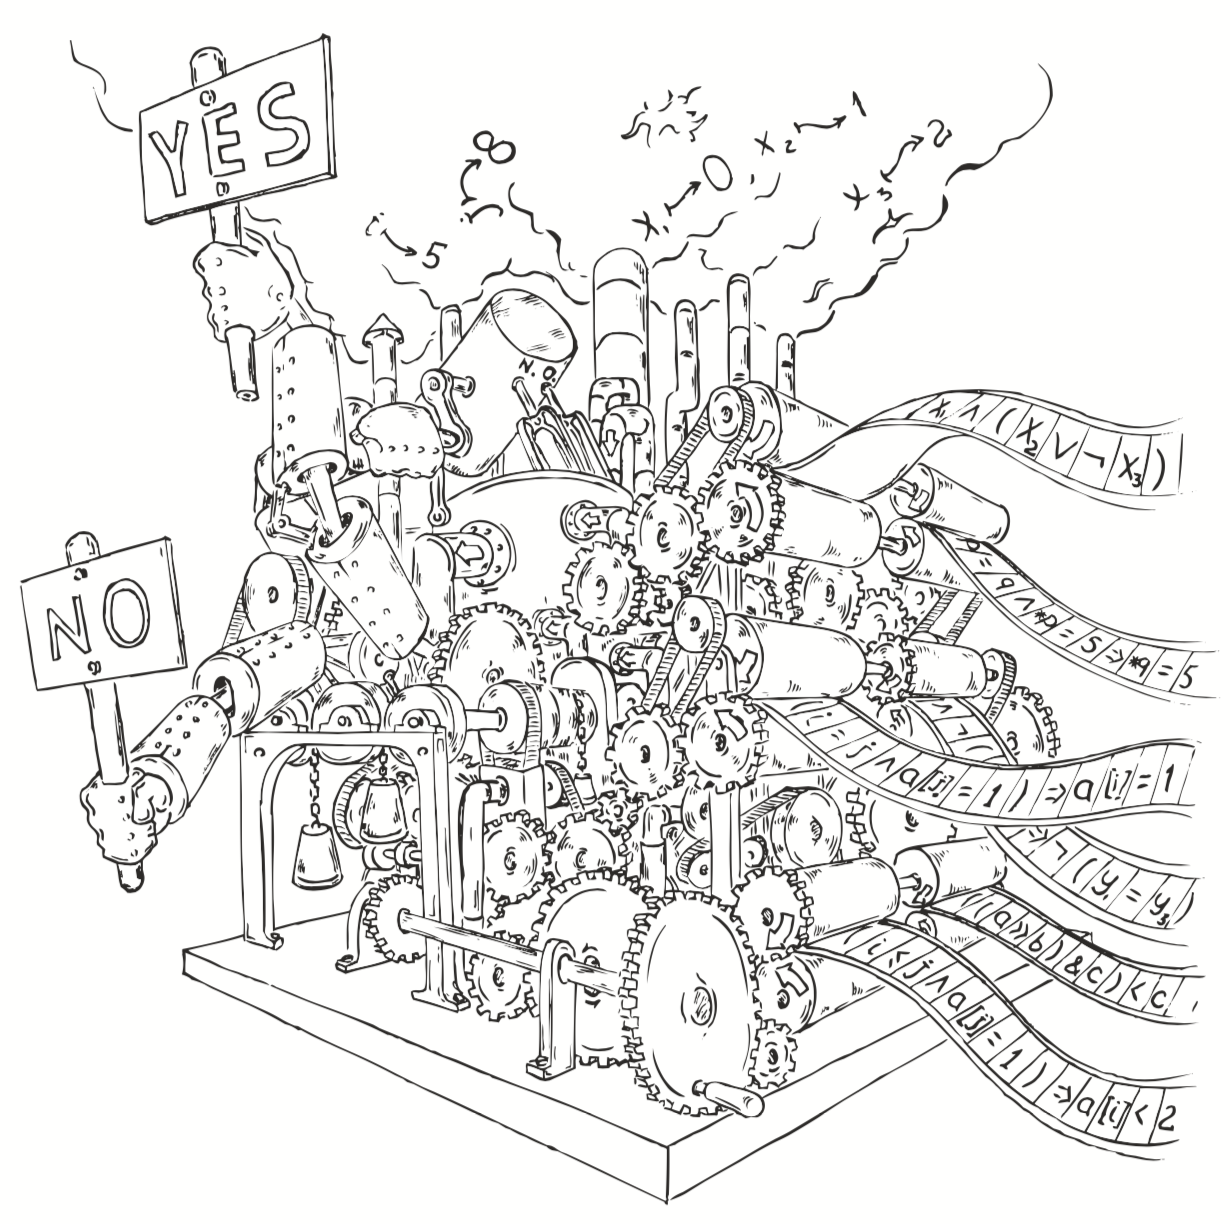
\includegraphics[scale=0.5]{../decision-procedure.png}
\end{frame}

\frame{\titlepage}

\begin{frame}{Предыдущая лекция: равновыполнимость}
\begin{itemize}
\item Выполнимость: $\phi$ - выполнима, если существуют такие значения переменных, входящих в $\phi$, что $\phi$ - истина.
\item Равновыполнимость: формулы $\phi1$ и $\phi2$ равновыполнимы, если $\phi1$ выполнима тогда и только тогда, когда $\phi2$
выполнима.
\end{itemize}
\end{frame}

\begin{frame}{Представления чисел}
\begin{itemize}
\item На прошлой лекции мы разобрали функцию AtMostOne
\end{itemize}
\end{frame}

\begin{frame}{Представления чисел}
\begin{itemize}
\item На прошлой лекции мы разобрали функцию AtMostOne
\item Как получить функцию AtMostK?
\end{itemize}
\end{frame}

\begin{frame}{Представления чисел}
\begin{itemize}
\item На прошлой лекции мы разобрали функцию AtMostOne
\item Унарное представление чисел:\newline
$x_n$ - истина, тогда и только тогда, когда число равно или больше n\newline
$x_i \rightarrow x_{i+1}: \bigwedge_{i<j}(\lnot x_i \vee x_j)$
\end{itemize}
\end{frame}

\begin{frame}{Представления чисел}
\begin{itemize}
\item На прошлой лекции мы разобрали функцию AtMostOne
\item Унарное представление чисел:\newline
$x_n$ - истина, тогда и только тогда, когда число равно или больше n\newline
$x_i \rightarrow x_{i+1}: \bigwedge_{i<j}(\lnot x_i \vee x_j)$
\item Бинарное представление:
Используя $O(log(n))$ битов можно представить число в бинарном виде
\end{itemize}
\end{frame}

\begin{frame}{Предыдущая лекция: Гамильтонов цикл}
\begin{itemize}
\item Что такое $\Sigma_{j} x_{ij} = 1$?
\end{itemize}
\end{frame}

\begin{frame}{Предыдущая лекция: Гамильтонов цикл}
\begin{itemize}
\item Что такое $\Sigma_{j} x_{ij} = 1$?
\item $AtMostOne(x_1, \dots, x_n) \wedge (x_1 \vee \dots \vee x_n)$
\end{itemize}
\end{frame}

\begin{frame}{Предыдущая лекция: Гамильтонов цикл}
\begin{itemize}
\item Что такое $\Sigma_{j} x_{ij} = 1$?
\item $AtMostOne(x_1, \dots, x_n) \wedge (x_1 \vee \dots \vee x_n)$
\item А $\Sigma_{ij \in S} x_{ij} \le |S| - 1$?
\end{itemize}
\end{frame}

\begin{frame}{Предыдущая лекция: Гамильтонов цикл}
\begin{itemize}
\item Что такое $\Sigma_{j} x_{ij} = 1$?
\item $AtMostOne(x_1, \dots, x_n) \wedge (x_1 \vee \dots \vee x_n)$
\item А $\Sigma_{ij \in S} x_{ij} \le |S| - 1$?
\item $AtMost(s - 1)(x_1, \dots, x_n)$
\end{itemize}
\end{frame}

\begin{frame}{Раскраска графа}
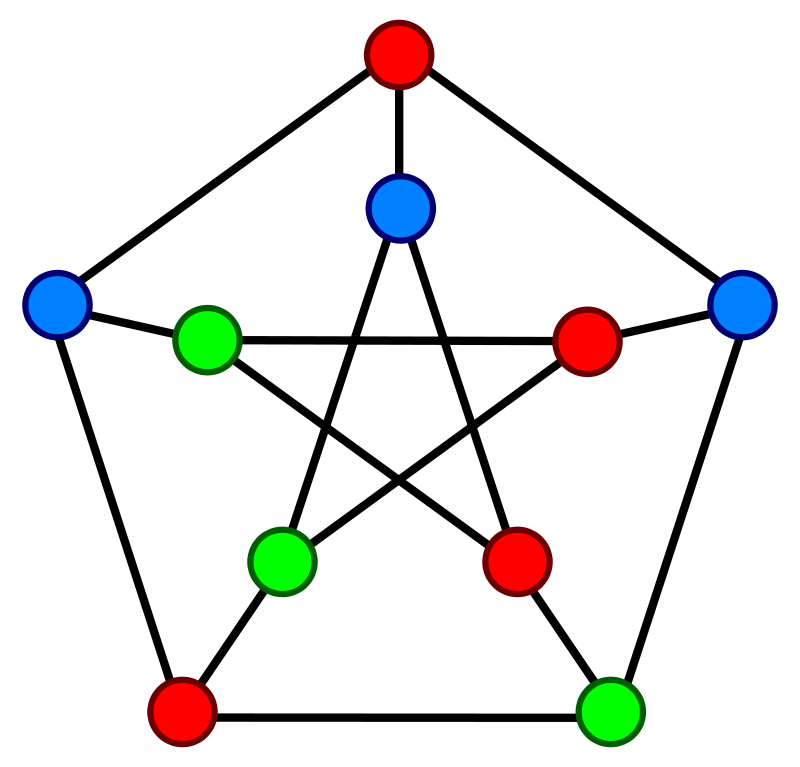
\includegraphics[scale=0.1]{graph-coloring.svg.png}
Имеется граф $G = (V, E)$. Можно ли его вершини расскрасить в $k$ цветов так, чтобы никакие соседние вершины не были раскрашены
в один и тот же цвет?
\end{frame}

\begin{frame}{Раскраска графа}
\begin{itemize}
\item Введем следующие переменные:\newline
$x_{v,i}$ - вершина $v$ имеет цвет $c$
\end{itemize}
\end{frame}

\begin{frame}{Раскраска графа}
\begin{itemize}
\item Введем следующие переменные:\newline
$x_{v,i}$ - вершина $v$ имеет цвет $c$
\item Уравнения:\newline
$(x_{v,1} \vee \dots \vee x_{v,c})$ - $v$ покрашена\newline
$(\lnot x_{v,s} \vee \lnot x_{v,t})$, $1 \le s \le c - 1$, $s + 1 \le t \le c$ - $v$ имеет не более одного цвета\newline
$(\lnot x_{v,i} \vee \lnot x_{w,i})$ - $v$ и $w$ имеют разный цвет
\end{itemize}
\end{frame}

\begin{frame}{Ферзь}
\begin{itemize}
\item Поставить на доску со стотронами $n\times n$ ферзей в количстве $n$ штук так, чтобы они не били друг друга.
\end{itemize}
\end{frame}

\begin{frame}{Ферзь}
\begin{itemize}
\item Поставить на доску со стотронами $n\times n$ ферзей в количстве $n$ штук так, чтобы они не били друг друга.
\item Уравнения:\newline
$ExeactlyOne(x_{1,j}, \dots x_{n, j})$ - ровно одна клетка в строке занята\newline
$ExeactlyOne(x_{1,j}, \dots x_{n, j})$ - ровно одна клетка в столбце занята\newline
$AtLeastOne(x_{i, j})$ для всех $i,j: i + j = k$ - ровно одна клетка на диагонали занята\newline
$AtLeastOne(x_{i, j})$ для всех $i,j: |i - j| = k$ - ровно одна клетка на диагонали занята\newline
\end{itemize}
\end{frame}

\begin{frame}{Теория первого порядка}
\begin{itemize}
\item Сигнатура $\Sigma = (R, F, C, \rho)$\newline
$R$ - множество символов для отношений (предикатов)\newline
$F$ - множество функциональных символов\newline
$C$ - множество констант\newline
Функция $\rho$, сопоставляющая элементам $R$ и $F$ их арность
\item Переменные
\item Логические операции: $\vee, \wedge, \rightarrow, \lnot$
\item Кванторы: $\forall, \exists$
\item Скобки, запятые
\end{itemize}
\end{frame}

\begin{frame}{Теория первого порядка}
\begin{itemize}
\item Терм - функциональный символ, либо $f(t_1, \dots, t_{\rho (f)})$, где $f$ - символ арности $\rho (f)$, $t_i$ - термы
\item Атом - $p(t_1, \dots t_{\rho (p)})$, где $p$ - предикатный символ арности $\rho (p)$, $t_i$ - термы
\item Формула - либо атом, либо $\lnot f_1$, $f_1 \vee f_2$, $f_1 \wedge f_2$, $f_1 \rightarrow f_2$, $\forall x f_1$,
$\exists x f_1$, где $f_1$ и $f_2$ - формулы
\end{itemize}
\end{frame}

\begin{frame}{Теория первого порядка}
\begin{itemize}
\item Задать модель:\newline
задать множество $D$ - домен\newline
задать функцию $\sigma$, т.ч. каждому предикатному символу сопоставляет предикат, функциональному символу сопоставляет функцию,
а константам сопоставлет элемент из $D$
\end{itemize}
\end{frame}

\begin{frame}{Теория первого порядка}
\begin{itemize}
\item Задать модель:\newline
задать множество $D$ - домен\newline
задать функцию $\sigma$, т.ч. каждому предикатному и функциональному символу сопоставить предикат и функцию
\item Пусть $s$ - функция, которая сопоставляет каждой переменной некоторое значение из $D$
\item Интерпретация формул относительно функции $s$ - индуктивно вычислить формулу.
\end{itemize}
\end{frame}

\begin{frame}
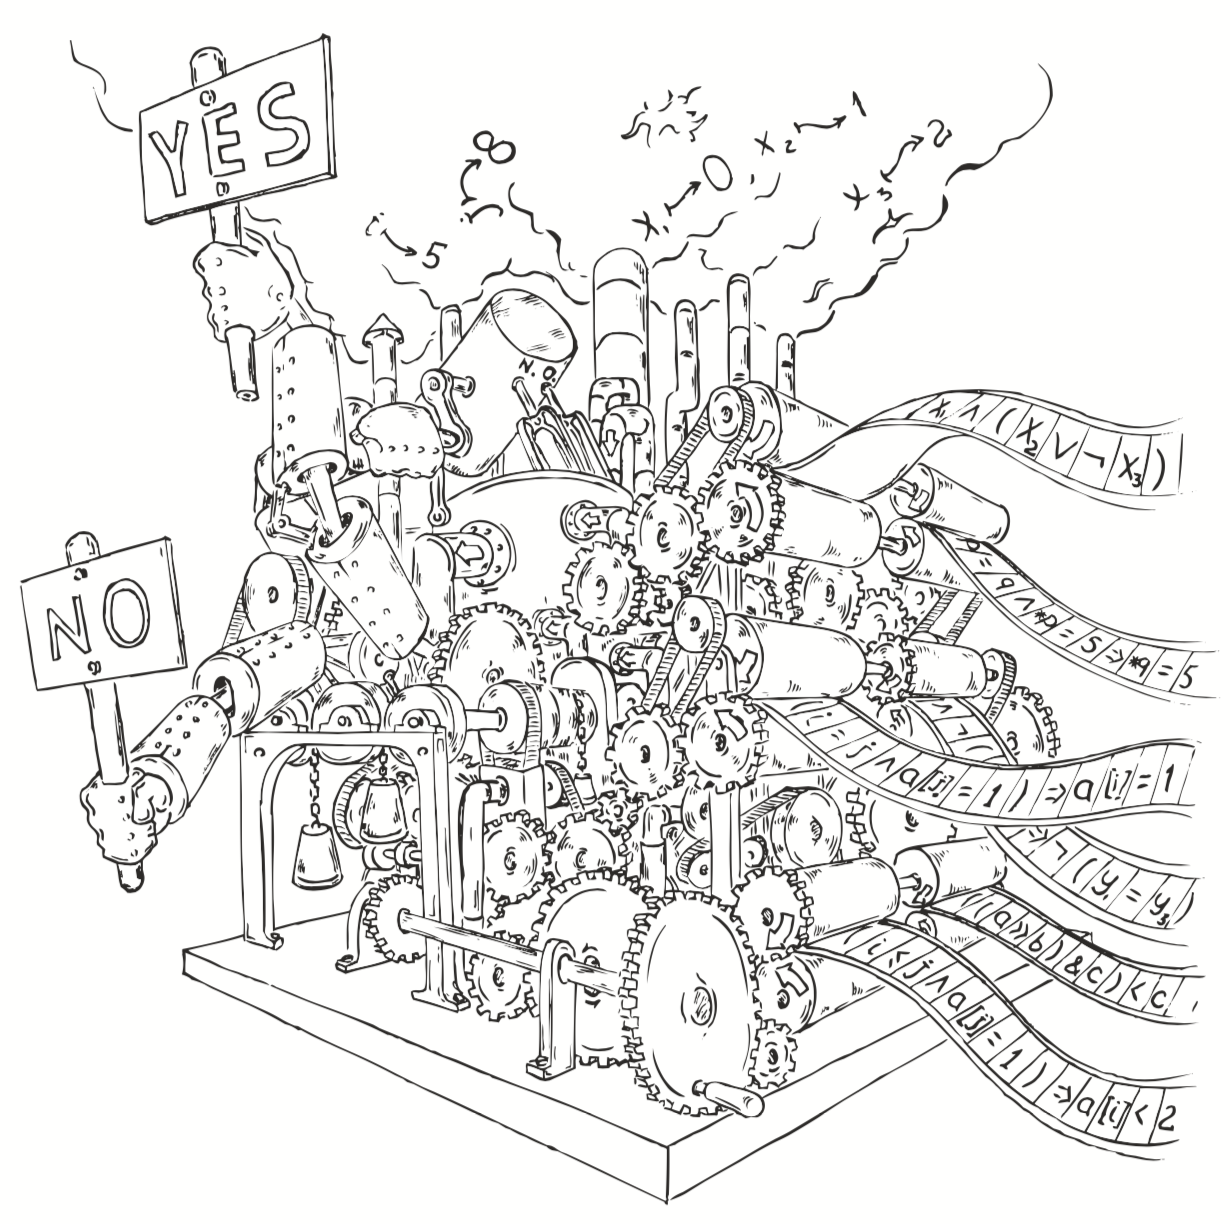
\includegraphics[scale=0.5]{../decision-procedure.png}
\end{frame}

\end{document}
